\documentclass[12pt,a4paper]{article}
\usepackage[left=0.5cm, right=0.5cm, top=0.5cm, bottom=0.5cm]{geometry}
\usepackage{pgfpages}
\usepackage{pdfpages}
\usepackage{amsmath, amssymb, esint}
\usepackage{booktabs} % For tables
\usepackage{graphicx} % For images
\usepackage{tikz}
\usetikzlibrary{shapes, calc}
\usepackage{pdflscape}
\usetikzlibrary{circuits.ee.IEC}

\pgfpagesdeclarelayout{4 on 1 reordered}
{
	\edef\pgfpageoptionheight{\the\paperheight} 
	\edef\pgfpageoptionwidth{\the\paperwidth}
	\def\pgfpageoptionborder{0 pt}
}
{
	\pgfpagesphysicalpageoptions
	{%
		logical pages=4,%
		physical height=\pgfpageoptionheight,%
		physical width=\pgfpageoptionwidth%
	}
	\pgfpageslogicalpageoptions{1}
	{%
		border shrink=\pgfpageoptionborder,%
		resized width=.5\pgfphysicalwidth,%
		resized height=.5\pgfphysicalheight,%
		center=\pgfpoint{.25\pgfphysicalwidth}{.75\pgfphysicalheight}%
	}%
	\pgfpageslogicalpageoptions{2}
	{%
		border shrink=\pgfpageoptionborder,%
		resized width=.5\pgfphysicalwidth,%
		resized height=.5\pgfphysicalheight,%
		center=\pgfpoint{.25\pgfphysicalwidth}{.25\pgfphysicalheight}%
	}%
	\pgfpageslogicalpageoptions{3}
	{%
		border shrink=\pgfpageoptionborder,%
		resized width=.5\pgfphysicalwidth,%
		resized height=.5\pgfphysicalheight,%
		center=\pgfpoint{.75\pgfphysicalwidth}{.75\pgfphysicalheight}%
	}%
	\pgfpageslogicalpageoptions{4}
	{%
		border shrink=\pgfpageoptionborder,%
		resized width=.5\pgfphysicalwidth,%
		resized height=.5\pgfphysicalheight,%
		center=\pgfpoint{.75\pgfphysicalwidth}{.25\pgfphysicalheight}%
	}%
}

\pgfpagesuselayout{4 on 1 reordered}[a4paper,border shrink=5mm]

\title{Physics Formula Sheet}
\author{402-0023-01L  Physics}
\date{2023/ 2024}

\begin{document}
	\maketitle
	
	\section*{Constants}
	\begin{tabular}{lll}
		\toprule
		Constant & Symbol & Value \\
		\midrule
		Speed of light & \( c \) & \( 3.00 \times 10^8 \) m/s \\
		Gravitational constant & \( G \) & \( 6.674 \times 10^{-11} \) N(m/kg)\(^2\) \\
		Planck's constant & \( h \) & \( 6.626 \times 10^{-34} \) J.s \\
		Mass of the electron & \( m_e \) & \( 9.10939 \times 10^{-31} \) kg \\
		Mass of the proton & \( m_p \) & \( 1.67262 \times 10^{-27} \) kg \\
		Charge of the electron & \(-e\) & \(-1.60218 \times 10^{-19} \) C \\
		Permittivity of free space & \(\epsilon_0\) & \( 8.85419 \times 10^{-12} \) C\(^2\)/J m \\
		Permeability of free space & \(\mu_0\) & \( 4 \pi \times 10^{-7} \) T m / A \\
		Boltzmann constant & \( k_B \) & \( 1.38066 \times 10^{-23} \) J/ K \\
		Avogadro's constant & \( N_A \) & \( 6.022 \times 10^{23} \) 1/mol \\
		\bottomrule
	\end{tabular}
	
	\section*{Oscillations}
	\subsection*{Equation of Motion}
	Undamped simple harmonic oscillator:
	\( 	m \frac{d^2 x}{dt^2} + kx = 0\)
	
	The equation of motion for a damped simple harmonic oscillator is:
	\[
	m \frac{d^2 x}{dt^2} + b \frac{dx}{dt} + kx = 0
	\]
	%Where:
	%\begin{itemize}
	%	\item \( m \) is the mass of the object.
	%	\item \( c \) is the damping coefficient.
	%	\item \( k \) is the spring constant.
	%	\item \( x \) is the displacement from the equilibrium position.
	%\end{itemize}
	
	\subsection*{General Solutions}
	\indent Light damping: (\( b^2 < 4mk \)), the general solution is:\\
	\[
	x(t) = e^{-\frac{b}{2m}t} \left( C_1 \cos(\omega_d t) + C_2 \sin(\omega_d t) \right)
	\]
	Where:
	\[
	\omega_d = \sqrt{\frac{k^2}{m^2} - \frac{b^2}{4m^2}}
	\]
	
	Critical camping: (\( b^2 = 4mk \)), the general solution is:\\
	\[
	x(t) = e^{-\frac{b}{2m}t} \left( C_1 + C_2 t \right)
	\]
	
	Heavy camping: (\( b^2 > 4mk \)), the general solution is:\\
	\[
	x(t) = e^{-\frac{b}{2m}t} \left( C_1 e^{\lambda_1} + C_2 e^{\lambda_2} \right)
	\]
	where \[ \lambda_{1,2} = -\frac{b}{2m} \pm \sqrt{\frac{b^2}{4m^2} - \frac{k^2}{m^2}} \]
	\subsection*{Graphs}
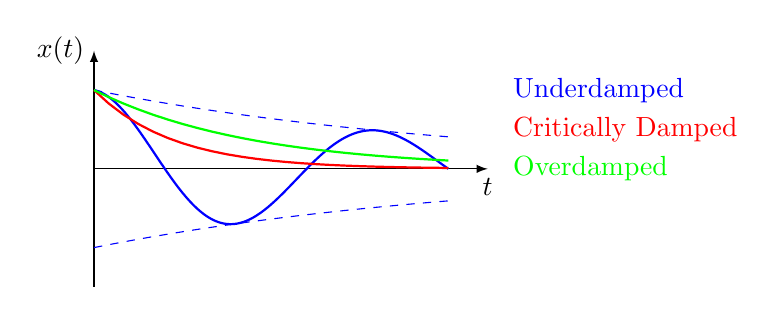
\begin{tikzpicture}
	% Axis
	\draw[-latex] (0,-1.5) -- (0,1.5) node[left] {$x(t)$};
	\draw[-latex] (0,0) -- (5,0) node[below] {$t$};
	
	% Oscillatory (Underdamped)
	\draw[blue, thick, domain=0:4.5, samples=500] plot (\x, {exp(-0.2*\x)*cos(100*\x)});
	\draw[blue, dashed, domain=0:4.5, samples=500] plot (\x, {exp(-0.2*\x)});
	\draw[blue, dashed, domain=0:4.5, samples=500] plot (\x, {-exp(-0.2*\x)});
	\node[blue, anchor=west] at (5.2,1) {Underdamped};
	
	% Critically Damped
	\draw[red, thick, domain=0:4.5] plot (\x, {exp(-\x)});
	\node[red, anchor=west] at (5.2,0.5) {Critically Damped};
	
	% Overdamped (Heavily Damped)
	\draw[green, thick, domain=0:4.5] plot (\x, {exp(-.5*\x)});
	\node[green, anchor=west] at (5.2,0) {Overdamped};
	
\end{tikzpicture}
	
	\subsection*{Energy}
	The energy of the system will decrease over time due to the dissipative forces (damping).
	
	\subsection*{Q Factor}
	The quality factor, or \( Q \) factor, describes the damping of the system:
	\[
	Q = \frac{1}{\frac{b}{2\sqrt{mk}}}
	\]
	A higher \( Q \) means the system is less damped.
	
	

	
\subsection*{Moments of Inertia}

Parallel axis theorem:
\begin{equation}
	I_O = I_{cg} + m d^2
\end{equation}
Perpendicular axis Theorem: 
\begin{equation}
	I_{z}=I_{x}+I_{y}
\end{equation}

\renewcommand{\arraystretch}{1.5} % Adjusts the spacing between table rows
\begin{tabular}{l|llc}
	\textbf{Object} & \textbf{Axis} & \textbf{Moment of Inertia (\( I \))} &\\
	\hline
	Thin cylindrical shell & Diameter through centre & \( \frac{1}{2} m r^2 + \frac{1}{12}ml^2\) & 		\includegraphics[width=2cm]{moiThinSphereDiam.pdf}\\
	\hline
	
	Thin cylindrical shell & Axis & \( mr^2\) & \includegraphics[width=2cm]{page0009.pdf}\\
	\hline
	
	Thin rod & End & \( \frac{1}{3} m l^2 \) &\includegraphics[width=2cm]{page0003.pdf}\\
	\hline
	
	Thin rod & Centre & \( \frac{1}{12} m l^2 \) &\includegraphics[width=2cm]{page0002.pdf}\\
	\hline
	
	Spherical shell & Centre & \( \frac{2}{3} m r^2 \) &\includegraphics[width=2cm]{page0011.pdf}\\
	\hline
	
	Solid sphere & Centre & \( \frac{2}{5} m r^2 \) &\includegraphics[width=2cm]{page0010.pdf}\\
	\hline
	
	Solid cylinder & Axis & \( \frac{1}{2} m r^2 \) &\includegraphics[width=2cm]{page0007.pdf}\\
	\hline
	
	Solid cylinder & Diameter through the centre& \( \frac{1}{4}m r^2 + \frac{1}{12}m l^2\) &\includegraphics[width=2cm]{moiSolidSphereDiam.pdf}\\
	\hline
	
	Hollow cylinder & Axis & \( \frac{1}{2}m (r_1^2+ r_2^2) \) &\includegraphics[width=2cm]{page0008.pdf}\\
	\hline
	
	Hollow cylinder & Diameter through centre & \( \frac{1}{4}m (r_1^2+ r_2^2) + \frac{1}{12}ml^2 \) &\includegraphics[width=2cm]{moiHollowSphereDiam.pdf}\\
	\hline
	
	Rectangular parallelpiped & Through centre, perpendicular to sides & \( \frac{1}{12} m (h^2 + w^2) \) &\includegraphics[width=2cm]{parallelpiped.pdf}\\
	
\end{tabular}


	
\section*{Thermodynamics}

\begin{quote}
\textbf{0th law:} 
If two objects are in thermal equilibrium with a third object, then all three objects are in thermal equilibrium with each other.
\end{quote}
\begin{quote}
\textbf{1st law:} 
For any process concerning a given system, the change in internal energy \(\Delta U\) of that system is equal to the sum of the heat \( Q \) transferred to that system and the work \( W \) performed on that system.
\[ \Delta U = Q + W \] , \[ dU = \delta Q + \delta W\]
\end{quote}

\begin{quote}
\textbf{2nd law:} 
\begin{itemize}
	\item \textbf{Carnot:} Wherever there exists a difference in temperature, motive power can be produced.
	\item \textbf{Kelvin:} It is impossible for a self-acting machine to convey heat from a colder body to a hotter one.
	\item \textbf{Clausius:} Heat cannot flow from a colder to a hotter body without another process occurring, connected therewith, simultaneously.
\end{itemize}
\end{quote}

Ideal gas law: \[ pV = NkT\]

\[
T = \left( \frac{\partial U}{\partial S} \right)_{V, N}
\]

Energy per degree of freedom: \[ \langle E_\text{mode} \rangle = \frac{1}{2} k_B T \]


Heat capacity, $C$: \[ Q = C \Delta T, \quad Q = \int_{T_1}^{T_2} C(T) \, dT \]

Latent heat, $L$: \[ L  = \frac{Q_\text{latent}}{m} \]


Isochoric process: \[ W = - \int P dV = 0\]
\[ \Delta Q = m C_V \Delta T\]

Isothermal process: \[ \Delta T = 0\]
\[ Q = \Delta U - W = - W = N k_B T_A \ln (\frac{V_B}{V_A})\]

Adiabatic process: \[ dU = \delta W\]

Adiabatic component: \[ \quad \gamma = \frac{C_P}{C_V} \]
Where P, V indicate at constant pressure/ volume

Polytropic equation for an adiabatic process: \[ pV^\gamma = \text{constant} \]

Efficiencies:\\
Heat engine: \( \eta = \frac{W}{Q_H}\)
Heat pump: \( \eta = \frac{Q_H}{W}\)
Fridge: \( \eta = \frac{Q_C}{W}\)



\subsection*{Electrostatics and dynamics}
	\setlength{\parskip}{.8em} % Adjusts the spacing between lines
	
	\[
	\mathbf{F} = \sum_{i=1}^{N} \frac{q_0 q_i (\mathbf{r}-\mathbf{r_i})}{4\pi \epsilon_0 |\mathbf{r}-\mathbf{r_i}|^3}
	\]
	
	Torque: \( \mathbf{\tau} = \mathbf{p} \times \mathbf{E} \)
	
	Energy of a dipole: \( U(\theta) = -\mathbf{p} \cdot \mathbf{E} \)
	
	Gauss' law: \( \phi = \oiint_{S} \mathbf{E} \cdot d\mathbf{A} \)
	
	Potential: \( \Delta V \equiv \frac{\Delta U}{q} = - \int_{C} \mathbf{E} \cdot d\mathbf{l} \)
	
	Energy of a capacitor: \( U = \frac{Q^2}{2C} \)
	
	Current: \( I = \dot{Q} \)
	
	Potential: \( V_b - V_a = -\int_{a}^{b} \mathbf{E} \cdot d\mathbf{l} \)
	
	Kirchhoff's rules:
	1. \( \sum_{j, \text{loop}} \Delta V_j = 0 \)
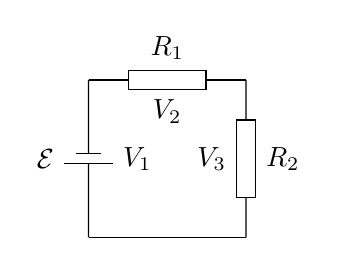
\begin{tikzpicture}[circuit ee IEC]
	% Drawing the battery (EMF) with positive and negative terminals
	\draw (0,0) to [battery={info={$\mathcal{E}$},info'={$V_1$}}] (0,2);
	
	% Drawing the resistors in the loop with voltage labels
	\draw (0,2) to [resistor={info={$R_1$},info'={$V_2$}},-*] (2,2);
	\draw (2,2) to [resistor={info={$R_2$},info'={$V_3$}}] (2,0);
	\draw (2,0) -- (0,0);
\end{tikzpicture}
	2. \( \sum_{j} I_{j, \text{into node}} = 0 \)
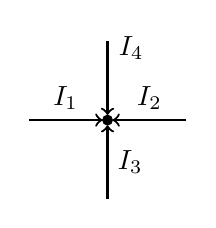
\begin{tikzpicture}[circuit ee IEC]
	% Drawing the node
	\node[contact] (N) at (0,0) {};
	
	% Drawing the current arrows and labels
	\draw[->, thick] (-1,0) -- (N) node[midway,above] {\(I_1\)};
	\draw[->, thick] (1,0) -- (N) node[midway,above] {\(I_2\)};
	\draw[->, thick] (0,-1) -- (N) node[midway,right] {\(I_3\)};
	\draw[->, thick] (0,1) -- (N) node[midway,above, xshift=0.3cm, yshift=0.1cm] {\(I_4\)};
\end{tikzpicture}

	
	Magnetic force: \( \mathbf{F} = q\mathbf{v} \times \mathbf{B} \)
	
	Cyclotron radius: \( r = \frac{mv}{qB} \)
	
	Biot-Savart: \( \mathbf{B} = \frac{\mu_0}{4 \pi} \cdot \frac{q \mathbf{v} \times \hat{r}}{r^2} \)
	
	Faraday's Law: \( \mathcal{E} = -\frac{d \phi_m}{dt} \)
	
	Self-inductance of a solenoid: \( L = \mu_0 n^2 A l \)
	
	Mutual inductance: \( \frac{\phi_{m1}}{N_1} = \frac{\phi_{m2}}{N_2} \)
	
	Impedance: \( Z_R = R, \, Z_C = \frac{1}{i \omega C}, \, Z_L = i \omega L \)
	
	
	\subsection*{Waves \& Quantum}
	\begin{align}
		\oint_{S} \mathbf{E} \cdot d\mathbf{A} &= \frac{Q_{\text{enc}}}{\epsilon_0} &\text{(Gauss's Law for Electricity)} \\
		\oint_{S} \mathbf{B} \cdot d\mathbf{A} &= 0 &\text{(Gauss's Law for Magnetism)} \\
		\oint_{C} \mathbf{E} \cdot d\mathbf{l} &= -\frac{d\Phi_{B}}{dt} &\text{(Faraday's Law)} \\
		\oint_{C} \mathbf{B} \cdot d\mathbf{l} &= \mu_0 I_{\text{enc}} + \mu_0 \epsilon_0 \frac{d\Phi_{E}}{dt} &\text{(Ampère's Law with Maxwell's addition)}
	\end{align}
	
	In electromagnetic waves, the ratio \( B_0 = \frac{E_0}{c} \) holds.
	
	Wavenumber: \( \omega = vk \)
	
	Compton wavelength: \( \lambda_c = \frac{h}{m_e c} \)
	
	Compton scattering: \( \Delta \lambda = \lambda_c (1-\cos \theta )\)
	
	De Broglie wavelength: \( \lambda_{\text{dB}} = \frac{h}{p} \)
	
	Heisenberg uncertainty relation: \( \Delta x \Delta p \geq \frac{h}{4\pi} \)
	
	Energy of a particle in a 1D box: \( E_n = \frac{h^2 n^2}{8L^2m} \)
	
	Energy of a photon: \( h \nu = E_m - E_n\)

	\begin{align*}
		\text{Time-dependent Schrodinger's Equation} & : i\hbar \frac{\partial}{\partial t} \Psi (\vec{x}, t) = [-\frac{\hbar^2}{2m}(\frac{\partial ^2}{\partial x^2} + \frac{\partial ^2}{\partial y ^2} + \frac{\partial^2}{\partial z^2}) + V(x)]\Psi (\vec{x}, t) \\
	\end{align*}
	
	\section*{Special relativity}
	Postulates of relativity and inertial reference frames:\\
	1: Absolute uniform motion cannot be detected.\\
	2: The speed of light in a vacuum is independent of the motion of the source.\\
	
	Time dilation: \( \Delta t = \gamma \Delta t_0\) \\
	
	Length contraction: \( L = \frac{L_0}{\gamma}\) \\
	
	\subsection*{Doppler Shift}
	
	\textbf{Non-relativistic Doppler Shift:}
	\begin{align}
		f' &= f \left( \frac{c \pm v_{\text{observer}}}{c \pm v_{\text{source}}} \right) \quad \text{(for sound or slow-moving sources)}
	\end{align}
	
	\textbf{Relativistic Doppler Shift:}
	\begin{align}
		f' &= f \sqrt{\frac{1 + \beta}{1 - \beta}} \quad \text{(for motion towards the observer)} \\
		f' &= f \sqrt{\frac{1 - \beta}{1 + \beta}} \quad \text{(for motion away from the observer)}
	\end{align}
	where \( \beta = \frac{v_{\text{source}}}{c} \).
	
	\subsection*{Velocity Transformations in Special Relativity}
	
	For two observers in relative motion with velocity \( v \) along the x-axis:
	
	\begin{align}
		u'_{x} &= \frac{u_{x} + v}{1 + \frac{vu_{x}}{c^2}} \\
		u'_{y} &= \frac{u_{y}}{\gamma(1 + \frac{vu_{x}}{c^2})} \\
		u'_{z} &= \frac{u_{z}}{\gamma(1 + \frac{vu_{x}}{c^2})}
	\end{align}
	
	where \( \gamma = \frac{1}{\sqrt{1 - \frac{v^2}{c^2}}} \) is the Lorentz factor.
	
	\subsection*{Energy}
	$\text{E}_\text{total} = \gamma mc^2 = \sqrt{p^2c^2 + m^2c^4}, \text{E}_\text{rest} = mc^2$
	
		
	\section*{Spherical coordinates}
	\[
		x = r \sin \theta \cos \phi,  y = r \sin \theta \sin \phi, z = r \cos \phi
	\]

	
	\vspace{.1in}
	Volume fraction: 
	\[ dV = r^2 \sin \theta dr d\theta d\phi \]
	
	\vspace{.1in}
	Solid angle: 
	\[ d\Omega = \frac{dS_r}{r^2} = \sin\theta d\theta d\phi \]
	
	\vspace{.1in}
	Surface element: 
	\[ dS_r = r^2 \sin\theta d\theta d\phi \]
	
	
	\begin{equation}
		\nabla f = \frac{\partial f}{\partial r} \vec{r} + \frac{1}{r} \frac{1}{r \sin \theta} \frac{\partial f}{\partial \phi} \vec{\phi}
	\end{equation}
	
	\begin{equation}
		\operatorname {div} \mathbf {F} =\nabla \cdot \mathbf {F} ={\frac {1}{r^{2}}}{\frac {\partial }{\partial r}}\left(r^{2}F_{r}\right)+{\frac {1}{r\sin \theta }}{\frac {\partial }{\partial \theta }}(\sin \theta \,F_{\theta })+{\frac {1}{r\sin \theta }}{\frac {\partial F_{\varphi }}{\partial \varphi }}.
	\end{equation}
	\begin{equation}
		\begin{aligned}
			\nabla \times \mathbf{F} = \frac{1}{r\sin\theta} (\frac{\partial }{\partial \theta} (A_\phi \sin \theta ) - \frac{\partial A_\theta}{\partial \phi}) \vec{r} \\
			+ \frac{1}{r}(\frac{1}{\sin\theta }\frac{\partial A_r}{\partial \phi} - \frac{\partial}{\partial r }(rA_\phi)) \vec{\theta} \\
			+ \frac{1}{r} (\frac{\partial}{\partial r}(r A_\phi) - \frac{\partial A_r}{\partial \phi}) \vec{\phi}
		\end{aligned}
	\end{equation}
	\begin{equation}
		\begin{aligned}
			\nabla^2 f = {1 \over r^{2}}{\partial  \over \partial r}\!\left(r^{2}{\partial f \over \partial r}\right)\!+\!{1 \over r^{2}\!\sin \theta }{\partial  \over \partial \theta }\!\left(\sin \theta {\partial f \over \partial \theta }\right)\!+\!{1 \over r^{2}\!\sin ^{2}\theta }{\partial ^{2}f \over \partial \varphi ^{2}} = \\ (\frac{\partial^2}{\partial r^2} + \frac{2}{r} \frac{\partial}{\partial r}) f
			+ \frac{1}{r^2 \sin \theta }\frac{\partial}{\partial \theta} (\sin \theta \frac{\partial}{\partial \theta})f
			+ \frac{1}{r^2 \sin ^2 \theta } \frac{\partial ^2}{\partial \phi ^2 } f
		\end{aligned}
	\end{equation}
	
	
	\section*{Inner product and expectation}
	\begin{center}
		Expectation value (discrete) \\[.15in]
		\(\langle f_i \rangle = \sum_{i} P_i f_i\) \\[.25in]
		Expectation value (continuous) \\[.15in]
		\(\langle f(x) \rangle = \int_{-\infty}^{\infty} f(x) P(x) \, dx\) \\[.15in]
		\(\langle \hat{O} \rangle = \int \psi^*(\mathbf{r}) \hat{O} \psi(\mathbf{r}) \, d^3r\) \\[.25in]
		Inner product \\[.15in]
		\(\langle \psi | \phi \rangle = \int \psi^*(x) \phi(x) \, dx\) \\[.25in]
		Variance \\[.15in]
		\(\sigma_f^2 = \langle f^2 \rangle - \langle f \rangle^2\)
	\end{center}	
	
	\begin{figure}
		\centering
		\includegraphics[width=0.7\linewidth]{latentHeat1}
		\caption{}
		\label{fig:latentheat2}
	\end{figure}
	
	\begin{figure}
		\centering
		\includegraphics[width=0.7\linewidth]{latentHeat2}
		\caption{}
		\label{fig:latentheat2}
	\end{figure}
	

	
\end{document}
